\documentclass[1p]{elsarticle_modified}
%\bibliographystyle{elsarticle-num}

%\usepackage[colorlinks]{hyperref}
%\usepackage{abbrmath_seonhwa} %\Abb, \Ascr, \Acal ,\Abf, \Afrak
\usepackage{amsfonts}
\usepackage{amssymb}
\usepackage{amsmath}
\usepackage{amsthm}
\usepackage{scalefnt}
\usepackage{amsbsy}
\usepackage{kotex}
\usepackage{caption}
\usepackage{subfig}
\usepackage{color}
\usepackage{graphicx}
\usepackage{xcolor} %% white, black, red, green, blue, cyan, magenta, yellow
\usepackage{float}
\usepackage{setspace}
\usepackage{hyperref}

\usepackage{tikz}
\usetikzlibrary{arrows}

\usepackage{multirow}
\usepackage{array} % fixed length table
\usepackage{hhline}

%%%%%%%%%%%%%%%%%%%%%
\makeatletter
\renewcommand*\env@matrix[1][\arraystretch]{%
	\edef\arraystretch{#1}%
	\hskip -\arraycolsep
	\let\@ifnextchar\new@ifnextchar
	\array{*\c@MaxMatrixCols c}}
\makeatother %https://tex.stackexchange.com/questions/14071/how-can-i-increase-the-line-spacing-in-a-matrix
%%%%%%%%%%%%%%%

\usepackage[normalem]{ulem}

\newcommand{\msout}[1]{\ifmmode\text{\sout{\ensuremath{#1}}}\else\sout{#1}\fi}
%SOURCE: \msout is \stkout macro in https://tex.stackexchange.com/questions/20609/strikeout-in-math-mode

\newcommand{\cancel}[1]{
	\ifmmode
	{\color{red}\msout{#1}}
	\else
	{\color{red}\sout{#1}}
	\fi
}

\newcommand{\add}[1]{
	{\color{blue}\uwave{#1}}
}

\newcommand{\replace}[2]{
	\ifmmode
	{\color{red}\msout{#1}}{\color{blue}\uwave{#2}}
	\else
	{\color{red}\sout{#1}}{\color{blue}\uwave{#2}}
	\fi
}

\newcommand{\Sol}{\mathcal{S}} %segment
\newcommand{\D}{D} %diagram
\newcommand{\A}{\mathcal{A}} %arc


%%%%%%%%%%%%%%%%%%%%%%%%%%%%%5 test

\def\sl{\operatorname{\textup{SL}}(2,\Cbb)}
\def\psl{\operatorname{\textup{PSL}}(2,\Cbb)}
\def\quan{\mkern 1mu \triangleright \mkern 1mu}

\theoremstyle{definition}
\newtheorem{thm}{Theorem}[section]
\newtheorem{prop}[thm]{Proposition}
\newtheorem{lem}[thm]{Lemma}
\newtheorem{ques}[thm]{Question}
\newtheorem{cor}[thm]{Corollary}
\newtheorem{defn}[thm]{Definition}
\newtheorem{exam}[thm]{Example}
\newtheorem{rmk}[thm]{Remark}
\newtheorem{alg}[thm]{Algorithm}

\newcommand{\I}{\sqrt{-1}}
\begin{document}

%\begin{frontmatter}
%
%\title{Boundary parabolic representations of knots up to 8 crossings}
%
%%% Group authors per affiliation:
%\author{Yunhi Cho} 
%\address{Department of Mathematics, University of Seoul, Seoul, Korea}
%\ead{yhcho@uos.ac.kr}
%
%
%\author{Seonhwa Kim} %\fnref{s_kim}}
%\address{Center for Geometry and Physics, Institute for Basic Science, Pohang, 37673, Korea}
%\ead{ryeona17@ibs.re.kr}
%
%\author{Hyuk Kim}
%\address{Department of Mathematical Sciences, Seoul National University, Seoul 08826, Korea}
%\ead{hyukkim@snu.ac.kr}
%
%\author{Seokbeom Yoon}
%\address{Department of Mathematical Sciences, Seoul National University, Seoul, 08826,  Korea}
%\ead{sbyoon15@snu.ac.kr}
%
%\begin{abstract}
%We find all boundary parabolic representation of knots up to 8 crossings.
%
%\end{abstract}
%\begin{keyword}
%    \MSC[2010] 57M25 
%\end{keyword}
%
%\end{frontmatter}

%\linenumbers
%\tableofcontents
%
\newcommand\colored[1]{\textcolor{white}{\rule[-0.35ex]{0.8em}{1.4ex}}\kern-0.8em\color{red} #1}%
%\newcommand\colored[1]{\textcolor{white}{ #1}\kern-2.17ex	\textcolor{white}{ #1}\kern-1.81ex	\textcolor{white}{ #1}\kern-2.15ex\color{red}#1	}

{\Large $\underline{10_{90}~(K10a_{92})}$}

\setlength{\tabcolsep}{10pt}
\renewcommand{\arraystretch}{1.6}
\vspace{1cm}\begin{tabular}{m{100pt}>{\centering\arraybackslash}m{274pt}}
\multirow{5}{120pt}{
	\centering
	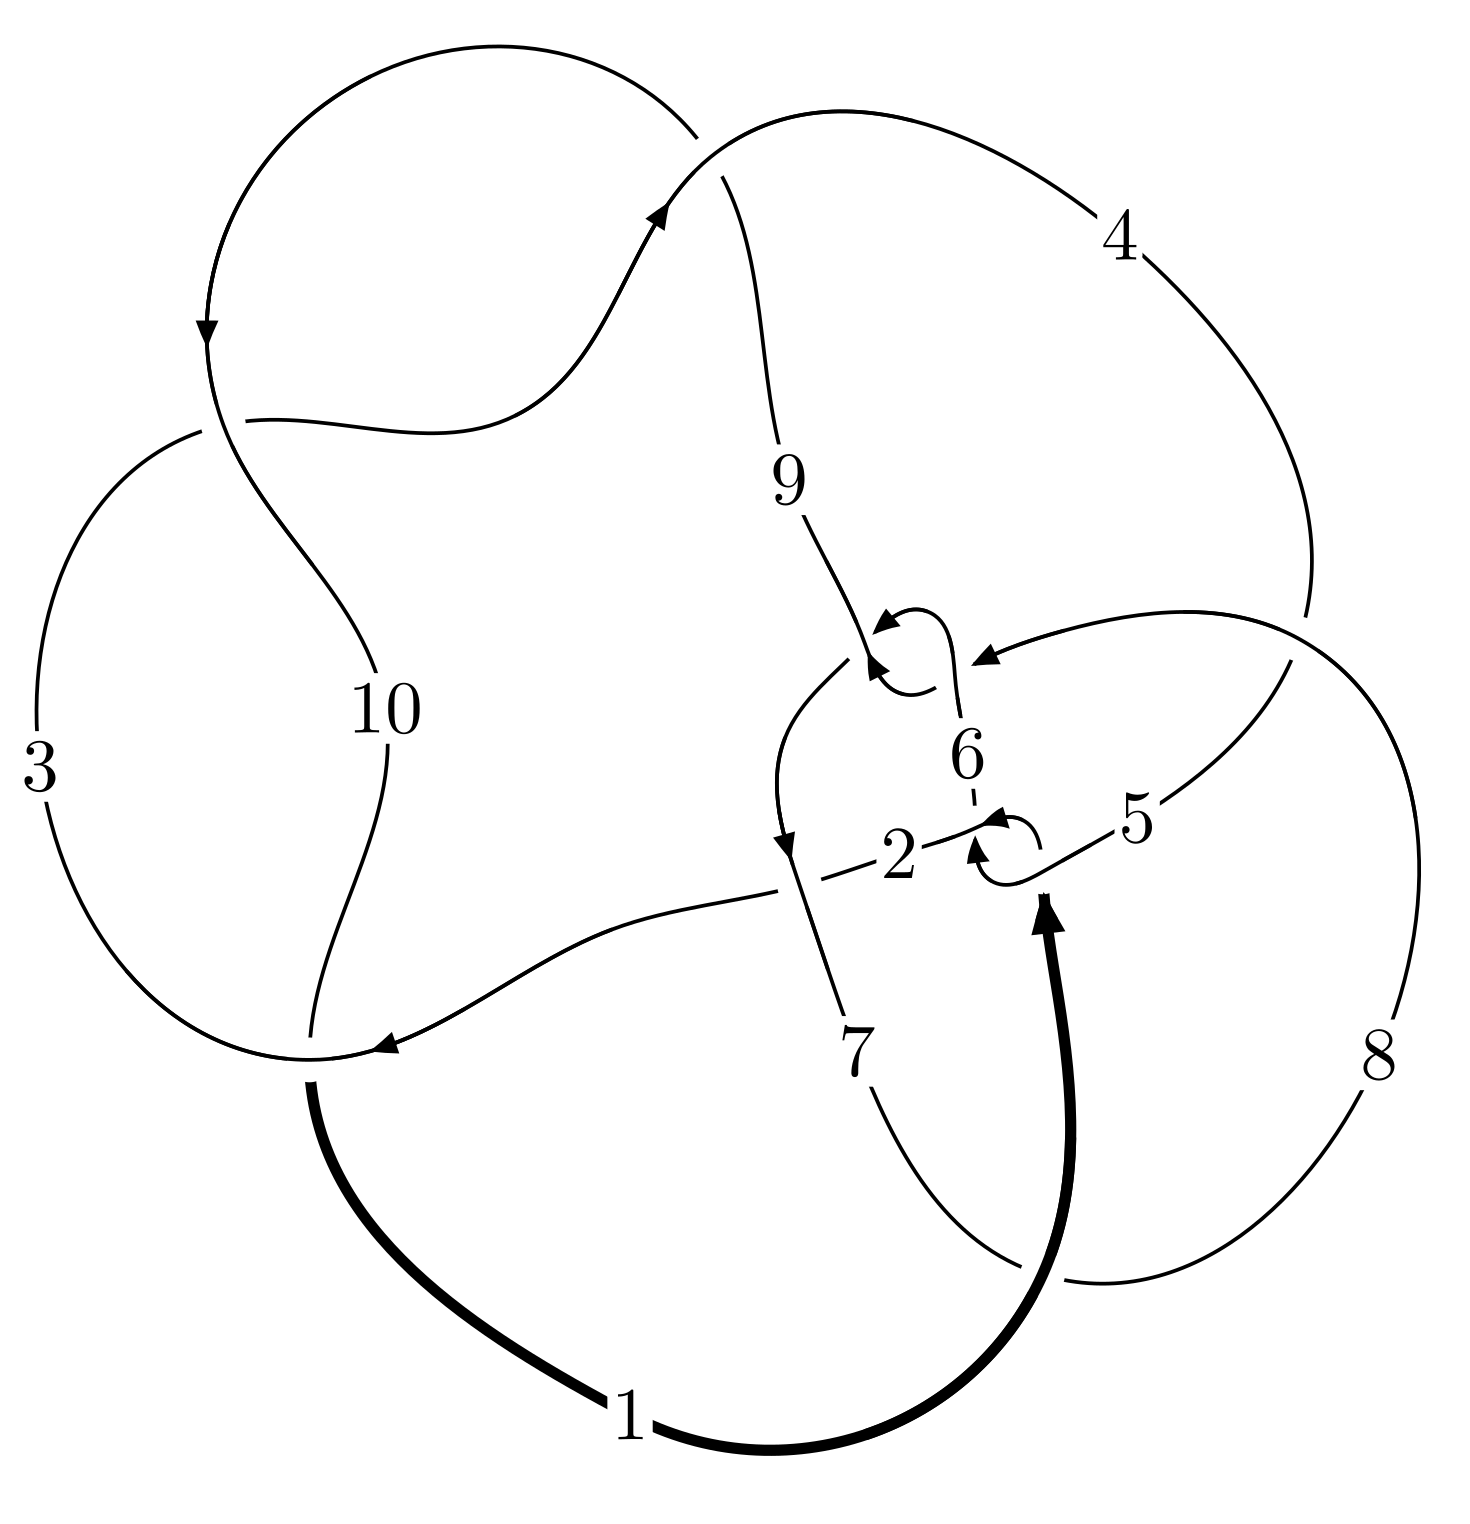
\includegraphics[width=112pt]{../../../GIT/diagram.site/Diagrams/png/174_10_90.png}\\
\ \ \ A knot diagram\footnotemark}&
\allowdisplaybreaks
\textbf{Linearized knot diagam} \\
\cline{2-2}
 &
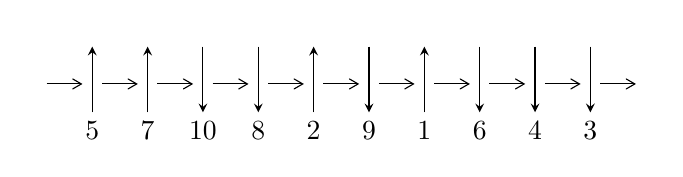
\begin{tikzpicture}[x=20pt, y=17pt]
	% nodes
	\node (C0) at (0, 0) {};
	\node (C1) at (1, 0) {};
	\node (C1U) at (1, +1) {};
	\node (C1D) at (1, -1) {5};

	\node (C2) at (2, 0) {};
	\node (C2U) at (2, +1) {};
	\node (C2D) at (2, -1) {7};

	\node (C3) at (3, 0) {};
	\node (C3U) at (3, +1) {};
	\node (C3D) at (3, -1) {10};

	\node (C4) at (4, 0) {};
	\node (C4U) at (4, +1) {};
	\node (C4D) at (4, -1) {8};

	\node (C5) at (5, 0) {};
	\node (C5U) at (5, +1) {};
	\node (C5D) at (5, -1) {2};

	\node (C6) at (6, 0) {};
	\node (C6U) at (6, +1) {};
	\node (C6D) at (6, -1) {9};

	\node (C7) at (7, 0) {};
	\node (C7U) at (7, +1) {};
	\node (C7D) at (7, -1) {1};

	\node (C8) at (8, 0) {};
	\node (C8U) at (8, +1) {};
	\node (C8D) at (8, -1) {6};

	\node (C9) at (9, 0) {};
	\node (C9U) at (9, +1) {};
	\node (C9D) at (9, -1) {4};

	\node (C10) at (10, 0) {};
	\node (C10U) at (10, +1) {};
	\node (C10D) at (10, -1) {3};
	\node (C11) at (11, 0) {};

	% arrows
	\draw[->,>={angle 60}]
	(C0) edge (C1) (C1) edge (C2) (C2) edge (C3) (C3) edge (C4) (C4) edge (C5) (C5) edge (C6) (C6) edge (C7) (C7) edge (C8) (C8) edge (C9) (C9) edge (C10) (C10) edge (C11) ;	\draw[->,>=stealth]
	(C1D) edge (C1U) (C2D) edge (C2U) (C3U) edge (C3D) (C4U) edge (C4D) (C5D) edge (C5U) (C6U) edge (C6D) (C7D) edge (C7U) (C8U) edge (C8D) (C9U) edge (C9D) (C10U) edge (C10D) ;
	\end{tikzpicture} \\
\hhline{~~} \\& 
\textbf{Solving Sequence} \\ \cline{2-2} 
 &
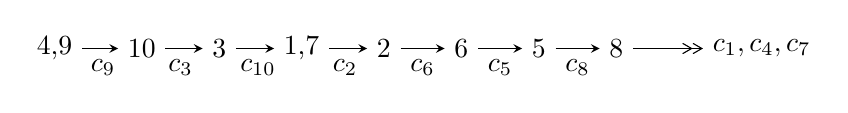
\begin{tikzpicture}[x=28pt, y=7pt]
	% node
	\node (A0) at (-1/8, 0) {4,9};
	\node (A1) at (1, 0) {10};
	\node (A2) at (2, 0) {3};
	\node (A3) at (49/16, 0) {1,7};
	\node (A4) at (33/8, 0) {2};
	\node (A5) at (41/8, 0) {6};
	\node (A6) at (49/8, 0) {5};
	\node (A7) at (57/8, 0) {8};
	\node (C1) at (1/2, -1) {$c_{9}$};
	\node (C2) at (3/2, -1) {$c_{3}$};
	\node (C3) at (5/2, -1) {$c_{10}$};
	\node (C4) at (29/8, -1) {$c_{2}$};
	\node (C5) at (37/8, -1) {$c_{6}$};
	\node (C6) at (45/8, -1) {$c_{5}$};
	\node (C7) at (53/8, -1) {$c_{8}$};
	\node (A8) at (9, 0) {$c_{1},c_{4},c_{7}$};

	% edge
	\draw[->,>=stealth]	
	(A0) edge (A1) (A1) edge (A2) (A2) edge (A3) (A3) edge (A4) (A4) edge (A5) (A5) edge (A6) (A6) edge (A7) ;
	\draw[->>,>={angle 60}]	
	(A7) edge (A8);
\end{tikzpicture} \\ 

\end{tabular} \\

\footnotetext{
The image of knot diagram is generated by the software ``\textbf{Draw programme}" developed by Andrew Bartholomew(\url{http://www.layer8.co.uk/maths/draw/index.htm\#Running-draw}), where we modified some parts for our purpose(\url{https://github.com/CATsTAILs/LinksPainter}).
}\phantom \\ \newline 
\centering \textbf{Ideals for irreducible components\footnotemark of $X_{\text{par}}$} 
 
\begin{align*}
I^u_{1}&=\langle 
-3.45798\times10^{19} u^{39}-4.51348\times10^{19} u^{38}+\cdots+2.27356\times10^{21} b+2.73076\times10^{21},\\
\phantom{I^u_{1}}&\phantom{= \langle  }-7.03658\times10^{21} u^{39}+1.13904\times10^{22} u^{38}+\cdots+6.82068\times10^{21} a+1.48581\times10^{21},\;u^{40}-2 u^{39}+\cdots-2 u+1\rangle \\
I^u_{2}&=\langle 
b+1,\;3 a-2 u+1,\;u^2- u+1\rangle \\
\\
\end{align*}
\raggedright * 2 irreducible components of $\dim_{\mathbb{C}}=0$, with total 42 representations.\\
\footnotetext{All coefficients of polynomials are rational numbers. But the coefficients are sometimes approximated in decimal forms when there is not enough margin.}
\newpage
\renewcommand{\arraystretch}{1}
\centering \section*{I. $I^u_{1}= \langle -3.46\times10^{19} u^{39}-4.51\times10^{19} u^{38}+\cdots+2.27\times10^{21} b+2.73\times10^{21},\;-7.04\times10^{21} u^{39}+1.14\times10^{22} u^{38}+\cdots+6.82\times10^{21} a+1.49\times10^{21},\;u^{40}-2 u^{39}+\cdots-2 u+1 \rangle$}
\flushleft \textbf{(i) Arc colorings}\\
\begin{tabular}{m{7pt} m{180pt} m{7pt} m{180pt} }
\flushright $a_{4}=$&$\begin{pmatrix}0\\u\end{pmatrix}$ \\
\flushright $a_{9}=$&$\begin{pmatrix}1\\0\end{pmatrix}$ \\
\flushright $a_{10}=$&$\begin{pmatrix}1\\u^2\end{pmatrix}$ \\
\flushright $a_{3}=$&$\begin{pmatrix}u\\u^3+u\end{pmatrix}$ \\
\flushright $a_{1}=$&$\begin{pmatrix}u^2+1\\u^4+2 u^2\end{pmatrix}$ \\
\flushright $a_{7}=$&$\begin{pmatrix}1.03165 u^{39}-1.66999 u^{38}+\cdots-9.20228 u-0.217839\\0.0152095 u^{39}+0.0198520 u^{38}+\cdots+0.294657 u-1.20110\end{pmatrix}$ \\
\flushright $a_{2}=$&$\begin{pmatrix}-1.20596 u^{39}+2.67703 u^{38}+\cdots-4.75631 u-2.57467\\0.765706 u^{39}-1.55826 u^{38}+\cdots+3.94732 u-1.22640\end{pmatrix}$ \\
\flushright $a_{6}=$&$\begin{pmatrix}1.04686 u^{39}-1.65014 u^{38}+\cdots-8.90762 u-1.41894\\0.0152095 u^{39}+0.0198520 u^{38}+\cdots+0.294657 u-1.20110\end{pmatrix}$ \\
\flushright $a_{5}=$&$\begin{pmatrix}-0.829665 u^{39}+2.71973 u^{38}+\cdots-11.3323 u-2.16330\\0.136920 u^{39}-0.520550 u^{38}+\cdots+3.27950 u-1.01464\end{pmatrix}$ \\
\flushright $a_{8}=$&$\begin{pmatrix}1.00098 u^{39}-1.67814 u^{38}+\cdots-9.29825 u-0.212902\\-0.101227 u^{39}+0.144212 u^{38}+\cdots-0.00592179 u-1.04475\end{pmatrix}$\\&\end{tabular}
\flushleft \textbf{(ii) Obstruction class $= -1$}\\~\\
\flushleft \textbf{(iii) Cusp Shapes $= -\frac{23709189092098357085641}{20462029573507327146753} u^{39}+\frac{5967042122571150693039}{2273558841500814127417} u^{38}+\cdots-\frac{151009571647058399841037}{6820676524502442382251} u+\frac{36425712582025581848210}{20462029573507327146753}$}\\~\\
\newpage\renewcommand{\arraystretch}{1}
\flushleft \textbf{(iv) u-Polynomials at the component}\newline \\
\begin{tabular}{m{50pt}|m{274pt}}
Crossings & \hspace{64pt}u-Polynomials at each crossing \\
\hline $$\begin{aligned}c_{1},c_{5}\end{aligned}$$&$\begin{aligned}
&u^{40}-2 u^{39}+\cdots-2 u+1
\end{aligned}$\\
\hline $$\begin{aligned}c_{2}\end{aligned}$$&$\begin{aligned}
&3(3 u^{40}+19 u^{39}+\cdots+64 u+32)
\end{aligned}$\\
\hline $$\begin{aligned}c_{3},c_{9},c_{10}\end{aligned}$$&$\begin{aligned}
&u^{40}-2 u^{39}+\cdots-2 u+1
\end{aligned}$\\
\hline $$\begin{aligned}c_{4}\end{aligned}$$&$\begin{aligned}
&3(3 u^{40}-10 u^{39}+\cdots-192 u+103)
\end{aligned}$\\
\hline $$\begin{aligned}c_{6},c_{8}\end{aligned}$$&$\begin{aligned}
&u^{40}-3 u^{39}+\cdots-31 u+9
\end{aligned}$\\
\hline $$\begin{aligned}c_{7}\end{aligned}$$&$\begin{aligned}
&u^{40}-3 u^{39}+\cdots-156 u+36
\end{aligned}$\\
\hline
\end{tabular}\\~\\
\newpage\renewcommand{\arraystretch}{1}
\flushleft \textbf{(v) Riley Polynomials at the component}\newline \\
\begin{tabular}{m{50pt}|m{274pt}}
Crossings & \hspace{64pt}Riley Polynomials at each crossing \\
\hline $$\begin{aligned}c_{1},c_{5}\end{aligned}$$&$\begin{aligned}
&y^{40}-22 y^{39}+\cdots-4 y+1
\end{aligned}$\\
\hline $$\begin{aligned}c_{2}\end{aligned}$$&$\begin{aligned}
&9(9 y^{40}-181 y^{39}+\cdots-13312 y+1024)
\end{aligned}$\\
\hline $$\begin{aligned}c_{3},c_{9},c_{10}\end{aligned}$$&$\begin{aligned}
&y^{40}+38 y^{39}+\cdots-4 y+1
\end{aligned}$\\
\hline $$\begin{aligned}c_{4}\end{aligned}$$&$\begin{aligned}
&9(9 y^{40}+38 y^{39}+\cdots+78084 y+10609)
\end{aligned}$\\
\hline $$\begin{aligned}c_{6},c_{8}\end{aligned}$$&$\begin{aligned}
&y^{40}-21 y^{39}+\cdots+389 y+81
\end{aligned}$\\
\hline $$\begin{aligned}c_{7}\end{aligned}$$&$\begin{aligned}
&y^{40}-15 y^{39}+\cdots-7416 y+1296
\end{aligned}$\\
\hline
\end{tabular}\\~\\
\newpage\flushleft \textbf{(vi) Complex Volumes and Cusp Shapes}
$$\begin{array}{c|c|c}  
\text{Solutions to }I^u_{1}& \I (\text{vol} + \sqrt{-1}CS) & \text{Cusp shape}\\
 \hline 
\begin{aligned}
u &= \phantom{-}0.718542 + 0.684654 I \\
a &= -0.109960 - 0.256762 I \\
b &= \phantom{-}1.052260 - 0.485181 I\end{aligned}
 & \phantom{-}1.29563 + 4.66233 I & -0.05723 - 4.37430 I \\ \hline\begin{aligned}
u &= \phantom{-}0.718542 - 0.684654 I \\
a &= -0.109960 + 0.256762 I \\
b &= \phantom{-}1.052260 + 0.485181 I\end{aligned}
 & \phantom{-}1.29563 - 4.66233 I & -0.05723 + 4.37430 I \\ \hline\begin{aligned}
u &= -0.875135 + 0.400189 I \\
a &= \phantom{-}0.674482 + 0.656422 I \\
b &= \phantom{-}1.057710 - 0.370943 I\end{aligned}
 & -2.73210 + 3.80447 I & -3.64129 - 6.83498 I \\ \hline\begin{aligned}
u &= -0.875135 - 0.400189 I \\
a &= \phantom{-}0.674482 - 0.656422 I \\
b &= \phantom{-}1.057710 + 0.370943 I\end{aligned}
 & -2.73210 - 3.80447 I & -3.64129 + 6.83498 I \\ \hline\begin{aligned}
u &= \phantom{-}0.812016 + 0.457171 I \\
a &= \phantom{-}0.695937 - 0.974226 I \\
b &= \phantom{-}1.221190 + 0.590650 I\end{aligned}
 & \phantom{-}0.61792 - 9.83239 I & -1.42359 + 7.89553 I \\ \hline\begin{aligned}
u &= \phantom{-}0.812016 - 0.457171 I \\
a &= \phantom{-}0.695937 + 0.974226 I \\
b &= \phantom{-}1.221190 - 0.590650 I\end{aligned}
 & \phantom{-}0.61792 + 9.83239 I & -1.42359 - 7.89553 I \\ \hline\begin{aligned}
u &= -0.668019 + 0.947602 I \\
a &= \phantom{-}0.128837 + 0.281540 I \\
b &= \phantom{-}0.847605 + 0.160546 I\end{aligned}
 & -1.20798 + 1.63374 I & \phantom{-}5.34484 + 3.65075 I \\ \hline\begin{aligned}
u &= -0.668019 - 0.947602 I \\
a &= \phantom{-}0.128837 - 0.281540 I \\
b &= \phantom{-}0.847605 - 0.160546 I\end{aligned}
 & -1.20798 - 1.63374 I & \phantom{-}5.34484 - 3.65075 I \\ \hline\begin{aligned}
u &= \phantom{-}0.548023 + 0.473980 I \\
a &= -0.128815 + 0.412875 I \\
b &= \phantom{-}0.217702 - 0.991146 I\end{aligned}
 & \phantom{-}3.67375 - 4.20324 I & \phantom{-}2.19223 + 6.09439 I \\ \hline\begin{aligned}
u &= \phantom{-}0.548023 - 0.473980 I \\
a &= -0.128815 - 0.412875 I \\
b &= \phantom{-}0.217702 + 0.991146 I\end{aligned}
 & \phantom{-}3.67375 + 4.20324 I & \phantom{-}2.19223 - 6.09439 I\\
 \hline 
 \end{array}$$\newpage$$\begin{array}{c|c|c}  
\text{Solutions to }I^u_{1}& \I (\text{vol} + \sqrt{-1}CS) & \text{Cusp shape}\\
 \hline 
\begin{aligned}
u &= \phantom{-}0.042556 + 1.284610 I \\
a &= \phantom{-}0.906133 + 0.658831 I \\
b &= -1.55343 - 0.24102 I\end{aligned}
 & \phantom{-}1.29749 - 1.62987 I & \phantom{-0.000000 -}0. + 3.54187 I \\ \hline\begin{aligned}
u &= \phantom{-}0.042556 - 1.284610 I \\
a &= \phantom{-}0.906133 - 0.658831 I \\
b &= -1.55343 + 0.24102 I\end{aligned}
 & \phantom{-}1.29749 + 1.62987 I & \phantom{-0.000000 } 0. - 3.54187 I \\ \hline\begin{aligned}
u &= \phantom{-}0.635260 + 0.284826 I \\
a &= \phantom{-}1.38094 - 0.39057 I \\
b &= \phantom{-}0.418271 + 0.528348 I\end{aligned}
 & \phantom{-}3.12136 + 0.50572 I & \phantom{-}2.23334 + 2.05026 I \\ \hline\begin{aligned}
u &= \phantom{-}0.635260 - 0.284826 I \\
a &= \phantom{-}1.38094 + 0.39057 I \\
b &= \phantom{-}0.418271 - 0.528348 I\end{aligned}
 & \phantom{-}3.12136 - 0.50572 I & \phantom{-}2.23334 - 2.05026 I \\ \hline\begin{aligned}
u &= \phantom{-}0.088735 + 1.341390 I \\
a &= \phantom{-}0.61542 + 1.56781 I \\
b &= -1.177540 - 0.538211 I\end{aligned}
 & \phantom{-}1.96980 - 1.69833 I & \phantom{-0.000000 } 0 \\ \hline\begin{aligned}
u &= \phantom{-}0.088735 - 1.341390 I \\
a &= \phantom{-}0.61542 - 1.56781 I \\
b &= -1.177540 + 0.538211 I\end{aligned}
 & \phantom{-}1.96980 + 1.69833 I & \phantom{-0.000000 } 0 \\ \hline\begin{aligned}
u &= -0.145572 + 1.361910 I \\
a &= \phantom{-}0.63895 - 1.93494 I \\
b &= -0.97948 + 1.02345 I\end{aligned}
 & \phantom{-}3.71762 + 5.12635 I & \phantom{-0.000000 } 0 \\ \hline\begin{aligned}
u &= -0.145572 - 1.361910 I \\
a &= \phantom{-}0.63895 + 1.93494 I \\
b &= -0.97948 - 1.02345 I\end{aligned}
 & \phantom{-}3.71762 - 5.12635 I & \phantom{-0.000000 } 0 \\ \hline\begin{aligned}
u &= -0.054010 + 1.410140 I \\
a &= \phantom{-}1.50150 - 2.72344 I \\
b &= -0.809247 + 0.079779 I\end{aligned}
 & \phantom{-}5.39390 + 0.19809 I & \phantom{-0.000000 } 0 \\ \hline\begin{aligned}
u &= -0.054010 - 1.410140 I \\
a &= \phantom{-}1.50150 + 2.72344 I \\
b &= -0.809247 - 0.079779 I\end{aligned}
 & \phantom{-}5.39390 - 0.19809 I & \phantom{-0.000000 } 0\\
 \hline 
 \end{array}$$\newpage$$\begin{array}{c|c|c}  
\text{Solutions to }I^u_{1}& \I (\text{vol} + \sqrt{-1}CS) & \text{Cusp shape}\\
 \hline 
\begin{aligned}
u &= \phantom{-}0.29805 + 1.43344 I \\
a &= \phantom{-}0.374682 - 1.281700 I \\
b &= \phantom{-}0.859448 + 0.587652 I\end{aligned}
 & \phantom{-}8.54985 - 3.07602 I & \phantom{-0.000000 } 0 \\ \hline\begin{aligned}
u &= \phantom{-}0.29805 - 1.43344 I \\
a &= \phantom{-}0.374682 + 1.281700 I \\
b &= \phantom{-}0.859448 - 0.587652 I\end{aligned}
 & \phantom{-}8.54985 + 3.07602 I & \phantom{-0.000000 } 0 \\ \hline\begin{aligned}
u &= -0.491071 + 0.191924 I \\
a &= -0.398403 - 1.001630 I \\
b &= -1.093680 + 0.645721 I\end{aligned}
 & -1.16688 + 2.84021 I & -5.40123 - 7.45362 I \\ \hline\begin{aligned}
u &= -0.491071 - 0.191924 I \\
a &= -0.398403 + 1.001630 I \\
b &= -1.093680 - 0.645721 I\end{aligned}
 & -1.16688 - 2.84021 I & -5.40123 + 7.45362 I \\ \hline\begin{aligned}
u &= -0.334189 + 0.406515 I \\
a &= \phantom{-}0.489517 - 0.524451 I \\
b &= -0.086689 + 0.335230 I\end{aligned}
 & -0.073174 + 1.047740 I & -1.21383 - 6.28305 I \\ \hline\begin{aligned}
u &= -0.334189 - 0.406515 I \\
a &= \phantom{-}0.489517 + 0.524451 I \\
b &= -0.086689 - 0.335230 I\end{aligned}
 & -0.073174 - 1.047740 I & -1.21383 + 6.28305 I \\ \hline\begin{aligned}
u &= -0.14754 + 1.48353 I \\
a &= -0.198631 - 1.161320 I \\
b &= \phantom{-}0.205553 + 0.846197 I\end{aligned}
 & \phantom{-}6.24860 + 2.92553 I & \phantom{-0.000000 } 0 \\ \hline\begin{aligned}
u &= -0.14754 - 1.48353 I \\
a &= -0.198631 + 1.161320 I \\
b &= \phantom{-}0.205553 - 0.846197 I\end{aligned}
 & \phantom{-}6.24860 - 2.92553 I & \phantom{-0.000000 } 0 \\ \hline\begin{aligned}
u &= \phantom{-}0.19425 + 1.47878 I \\
a &= -0.63962 + 1.50949 I \\
b &= \phantom{-}0.365197 - 1.279800 I\end{aligned}
 & \phantom{-}10.00150 - 6.93788 I & \phantom{-0.000000 } 0 \\ \hline\begin{aligned}
u &= \phantom{-}0.19425 - 1.47878 I \\
a &= -0.63962 - 1.50949 I \\
b &= \phantom{-}0.365197 + 1.279800 I\end{aligned}
 & \phantom{-}10.00150 + 6.93788 I & \phantom{-0.000000 } 0\\
 \hline 
 \end{array}$$\newpage$$\begin{array}{c|c|c}  
\text{Solutions to }I^u_{1}& \I (\text{vol} + \sqrt{-1}CS) & \text{Cusp shape}\\
 \hline 
\begin{aligned}
u &= -0.31725 + 1.49380 I \\
a &= -0.15513 + 1.42791 I \\
b &= \phantom{-}1.180340 - 0.563412 I\end{aligned}
 & \phantom{-}3.39122 + 8.09434 I & \phantom{-0.000000 } 0 \\ \hline\begin{aligned}
u &= -0.31725 - 1.49380 I \\
a &= -0.15513 - 1.42791 I \\
b &= \phantom{-}1.180340 + 0.563412 I\end{aligned}
 & \phantom{-}3.39122 - 8.09434 I & \phantom{-0.000000 } 0 \\ \hline\begin{aligned}
u &= \phantom{-}0.29587 + 1.50669 I \\
a &= -0.25279 - 1.73575 I \\
b &= \phantom{-}1.29708 + 0.71454 I\end{aligned}
 & \phantom{-}6.9750 - 13.8661 I & \phantom{-0.000000 } 0 \\ \hline\begin{aligned}
u &= \phantom{-}0.29587 - 1.50669 I \\
a &= -0.25279 + 1.73575 I \\
b &= \phantom{-}1.29708 - 0.71454 I\end{aligned}
 & \phantom{-}6.9750 + 13.8661 I & \phantom{-0.000000 } 0 \\ \hline\begin{aligned}
u &= \phantom{-}0.16112 + 1.56360 I \\
a &= -0.602788 + 0.551528 I \\
b &= \phantom{-}0.727804 - 0.598256 I\end{aligned}
 & \phantom{-}8.93627 + 1.59631 I & \phantom{-0.000000 } 0 \\ \hline\begin{aligned}
u &= \phantom{-}0.16112 - 1.56360 I \\
a &= -0.602788 - 0.551528 I \\
b &= \phantom{-}0.727804 + 0.598256 I\end{aligned}
 & \phantom{-}8.93627 - 1.59631 I & \phantom{-0.000000 } 0 \\ \hline\begin{aligned}
u &= \phantom{-}0.424864 + 0.027630 I \\
a &= -1.51964 + 0.31762 I \\
b &= -1.269680 - 0.070813 I\end{aligned}
 & -2.32372 - 0.01230 I & -6.85568 - 1.19794 I \\ \hline\begin{aligned}
u &= \phantom{-}0.424864 - 0.027630 I \\
a &= -1.51964 - 0.31762 I \\
b &= -1.269680 + 0.070813 I\end{aligned}
 & -2.32372 + 0.01230 I & -6.85568 + 1.19794 I \\ \hline\begin{aligned}
u &= -0.186501 + 0.360437 I \\
a &= \phantom{-}3.93271 - 1.95945 I \\
b &= -0.980417 - 0.195912 I\end{aligned}
 & -0.113312 - 0.691322 I & \phantom{-}2.03417 - 9.81182 I \\ \hline\begin{aligned}
u &= -0.186501 - 0.360437 I \\
a &= \phantom{-}3.93271 + 1.95945 I \\
b &= -0.980417 + 0.195912 I\end{aligned}
 & -0.113312 + 0.691322 I & \phantom{-}2.03417 + 9.81182 I\\
 \hline 
 \end{array}$$\newpage\newpage\renewcommand{\arraystretch}{1}
\centering \section*{II. $I^u_{2}= \langle b+1,\;3 a-2 u+1,\;u^2- u+1 \rangle$}
\flushleft \textbf{(i) Arc colorings}\\
\begin{tabular}{m{7pt} m{180pt} m{7pt} m{180pt} }
\flushright $a_{4}=$&$\begin{pmatrix}0\\u\end{pmatrix}$ \\
\flushright $a_{9}=$&$\begin{pmatrix}1\\0\end{pmatrix}$ \\
\flushright $a_{10}=$&$\begin{pmatrix}1\\u-1\end{pmatrix}$ \\
\flushright $a_{3}=$&$\begin{pmatrix}u\\u-1\end{pmatrix}$ \\
\flushright $a_{1}=$&$\begin{pmatrix}u\\u-2\end{pmatrix}$ \\
\flushright $a_{7}=$&$\begin{pmatrix}\frac{2}{3} u-\frac{1}{3}\\-1\end{pmatrix}$ \\
\flushright $a_{2}=$&$\begin{pmatrix}u+\frac{1}{3}\\\frac{5}{3} u-\frac{4}{3}\end{pmatrix}$ \\
\flushright $a_{6}=$&$\begin{pmatrix}\frac{2}{3} u-\frac{4}{3}\\-1\end{pmatrix}$ \\
\flushright $a_{5}=$&$\begin{pmatrix}\frac{1}{3} u\\\frac{4}{3} u-\frac{2}{3}\end{pmatrix}$ \\
\flushright $a_{8}=$&$\begin{pmatrix}\frac{2}{3} u-\frac{1}{3}\\-1\end{pmatrix}$\\&\end{tabular}
\flushleft \textbf{(ii) Obstruction class $= 1$}\\~\\
\flushleft \textbf{(iii) Cusp Shapes $= \frac{20}{3} u-9$}\\~\\
\newpage\renewcommand{\arraystretch}{1}
\flushleft \textbf{(iv) u-Polynomials at the component}\newline \\
\begin{tabular}{m{50pt}|m{274pt}}
Crossings & \hspace{64pt}u-Polynomials at each crossing \\
\hline $$\begin{aligned}c_{1},c_{3}\end{aligned}$$&$\begin{aligned}
&u^2+u+1
\end{aligned}$\\
\hline $$\begin{aligned}c_{2}\end{aligned}$$&$\begin{aligned}
&3(3 u^2+1)
\end{aligned}$\\
\hline $$\begin{aligned}c_{4}\end{aligned}$$&$\begin{aligned}
&3(3 u^2-3 u+1)
\end{aligned}$\\
\hline $$\begin{aligned}c_{5},c_{9},c_{10}\end{aligned}$$&$\begin{aligned}
&u^2- u+1
\end{aligned}$\\
\hline $$\begin{aligned}c_{6}\end{aligned}$$&$\begin{aligned}
&(u-1)^2
\end{aligned}$\\
\hline $$\begin{aligned}c_{7}\end{aligned}$$&$\begin{aligned}
&u^2
\end{aligned}$\\
\hline $$\begin{aligned}c_{8}\end{aligned}$$&$\begin{aligned}
&(u+1)^2
\end{aligned}$\\
\hline
\end{tabular}\\~\\
\newpage\renewcommand{\arraystretch}{1}
\flushleft \textbf{(v) Riley Polynomials at the component}\newline \\
\begin{tabular}{m{50pt}|m{274pt}}
Crossings & \hspace{64pt}Riley Polynomials at each crossing \\
\hline $$\begin{aligned}c_{1},c_{3},c_{5}\\c_{9},c_{10}\end{aligned}$$&$\begin{aligned}
&y^2+y+1
\end{aligned}$\\
\hline $$\begin{aligned}c_{2}\end{aligned}$$&$\begin{aligned}
&9(3 y+1)^2
\end{aligned}$\\
\hline $$\begin{aligned}c_{4}\end{aligned}$$&$\begin{aligned}
&9(9 y^2-3 y+1)
\end{aligned}$\\
\hline $$\begin{aligned}c_{6},c_{8}\end{aligned}$$&$\begin{aligned}
&(y-1)^2
\end{aligned}$\\
\hline $$\begin{aligned}c_{7}\end{aligned}$$&$\begin{aligned}
&y^2
\end{aligned}$\\
\hline
\end{tabular}\\~\\
\newpage\flushleft \textbf{(vi) Complex Volumes and Cusp Shapes}
$$\begin{array}{c|c|c}  
\text{Solutions to }I^u_{2}& \I (\text{vol} + \sqrt{-1}CS) & \text{Cusp shape}\\
 \hline 
\begin{aligned}
u &= \phantom{-}0.500000 + 0.866025 I \\
a &= \phantom{-0.000000 -}0.577350 I \\
b &= -1.00000\phantom{ +0.000000I}\end{aligned}
 & -1.64493 - 2.02988 I & -5.66667 + 5.77350 I \\ \hline\begin{aligned}
u &= \phantom{-}0.500000 - 0.866025 I \\
a &= \phantom{-0.000000 } -0.577350 I \\
b &= -1.00000\phantom{ +0.000000I}\end{aligned}
 & -1.64493 + 2.02988 I & -5.66667 - 5.77350 I\\
 \hline 
 \end{array}$$\newpage
\newpage\renewcommand{\arraystretch}{1}
\centering \section*{ III. u-Polynomials}
\begin{tabular}{m{50pt}|m{274pt}}
Crossings & \hspace{64pt}u-Polynomials at each crossing \\
\hline $$\begin{aligned}c_{1}\end{aligned}$$&$\begin{aligned}
&(u^2+u+1)(u^{40}-2 u^{39}+\cdots-2 u+1)
\end{aligned}$\\
\hline $$\begin{aligned}c_{2}\end{aligned}$$&$\begin{aligned}
&9(3 u^2+1)(3 u^{40}+19 u^{39}+\cdots+64 u+32)
\end{aligned}$\\
\hline $$\begin{aligned}c_{3}\end{aligned}$$&$\begin{aligned}
&(u^2+u+1)(u^{40}-2 u^{39}+\cdots-2 u+1)
\end{aligned}$\\
\hline $$\begin{aligned}c_{4}\end{aligned}$$&$\begin{aligned}
&9(3 u^2-3 u+1)(3 u^{40}-10 u^{39}+\cdots-192 u+103)
\end{aligned}$\\
\hline $$\begin{aligned}c_{5}\end{aligned}$$&$\begin{aligned}
&(u^2- u+1)(u^{40}-2 u^{39}+\cdots-2 u+1)
\end{aligned}$\\
\hline $$\begin{aligned}c_{6}\end{aligned}$$&$\begin{aligned}
&((u-1)^2)(u^{40}-3 u^{39}+\cdots-31 u+9)
\end{aligned}$\\
\hline $$\begin{aligned}c_{7}\end{aligned}$$&$\begin{aligned}
&u^2(u^{40}-3 u^{39}+\cdots-156 u+36)
\end{aligned}$\\
\hline $$\begin{aligned}c_{8}\end{aligned}$$&$\begin{aligned}
&((u+1)^2)(u^{40}-3 u^{39}+\cdots-31 u+9)
\end{aligned}$\\
\hline $$\begin{aligned}c_{9},c_{10}\end{aligned}$$&$\begin{aligned}
&(u^2- u+1)(u^{40}-2 u^{39}+\cdots-2 u+1)
\end{aligned}$\\
\hline
\end{tabular}\newpage\renewcommand{\arraystretch}{1}
\centering \section*{ IV. Riley Polynomials}
\begin{tabular}{m{50pt}|m{274pt}}
Crossings & \hspace{64pt}Riley Polynomials at each crossing \\
\hline $$\begin{aligned}c_{1},c_{5}\end{aligned}$$&$\begin{aligned}
&(y^2+y+1)(y^{40}-22 y^{39}+\cdots-4 y+1)
\end{aligned}$\\
\hline $$\begin{aligned}c_{2}\end{aligned}$$&$\begin{aligned}
&81(3 y+1)^2(9 y^{40}-181 y^{39}+\cdots-13312 y+1024)
\end{aligned}$\\
\hline $$\begin{aligned}c_{3},c_{9},c_{10}\end{aligned}$$&$\begin{aligned}
&(y^2+y+1)(y^{40}+38 y^{39}+\cdots-4 y+1)
\end{aligned}$\\
\hline $$\begin{aligned}c_{4}\end{aligned}$$&$\begin{aligned}
&81(9 y^2-3 y+1)(9 y^{40}+38 y^{39}+\cdots+78084 y+10609)
\end{aligned}$\\
\hline $$\begin{aligned}c_{6},c_{8}\end{aligned}$$&$\begin{aligned}
&((y-1)^2)(y^{40}-21 y^{39}+\cdots+389 y+81)
\end{aligned}$\\
\hline $$\begin{aligned}c_{7}\end{aligned}$$&$\begin{aligned}
&y^2(y^{40}-15 y^{39}+\cdots-7416 y+1296)
\end{aligned}$\\
\hline
\end{tabular}
\vskip 2pc
\end{document}